\documentclass[aspectratio=169,
				xcolor=table]{beamer}

% Load general definitions
\usepackage[utf8]{inputenc}
%\usepackage[T1]{fontenc}
\usepackage[brazil]{babel}
\usepackage{amsmath}
\usepackage{amsfonts}
\usepackage{amssymb}
\usepackage{graphicx}
\usepackage{verbatim}
\usepackage{cancel}
\usepackage{askmaps}
\usepackage{tabularx}
\usepackage[table]{xcolor}
%\usepackage{tikz}
\usepackage{multirow}
\usepackage{mathtools}
\usepackage{color, colortbl}
\usepackage{etoolbox}
\usepackage{pbox}
\usepackage{changepage}
\usepackage{xpatch}
\usepackage{array}
\usepackage{marvosym}
\usepackage{tabu}
\usepackage{multicol}
\usepackage{listings}
\usepackage{underscore}
\usepackage{filecontents}
\usepackage[]{algorithm2e}
\usepackage{ragged2e}

\newcolumntype{P}[1]{>{\centering\arraybackslash}m{#1}}
\definecolor{Gray}{gray}{0.75}
\definecolor{Gray2}{gray}{0.85}

\definecolor{lightBlue}{HTML}{DAE8FC}
\definecolor{Blue}{RGB}{51, 51, 204}

%\useinnertheme[lily]{rounded}
\usetheme{UniEvangelica}
%\usetheme{Copenhagen}
%\usetheme{Berlin}
%\usecolortheme{dolphin}
\tolerance=1
\emergencystretch=\maxdimen
\hyphenpenalty=10000
\hbadness=10000

\setbeamertemplate{navigation symbols}{}%remove navigation symbols


\let\olditem=\item% 
\renewcommand{\item}{\olditem \justifying}%
\def\center{\trivlist \centering\item\relax}
\def\endcenter{\endtrivlist}

\setbeamertemplate{itemize/enumerate body begin}{\large}
\setbeamertemplate{itemize/enumerate subbody begin}{\large}

\setbeamertemplate{itemize item}{\raisebox{0.1ex}{$\blacktriangleright$}\hskip0.1em}
\setbeamertemplate{itemize subitem}{\raisebox{0.1ex}{$\blacktriangleright$}\hskip0.1em}

\newcommand{\greenarrow}{\textcolor{green}{\rotatebox[origin=c]{180}{\MVArrowDown}}}

\newcommand{\redarrow}{\textcolor{red}{\MVArrowDown}}

%\newcommand{\ftable}{
%	\begin{table}
%		\large
%		\centering
%		\rowcolors{1}{\ifnumless{\rownum}{2}{Blue}{lightBlue}}{}
%}

\newenvironment{eftable}{
	\begin{table}
		\large
		\centering
		\rowcolors{1}{}{Blue}
		\rowcolors{1}{\ifnumless{\rownum}{2}{Blue}{lightBlue}}{}
	}
	{
	\end{table}
}


%\setbeamertemplate{frametitle}
%{
%	%\vspace*{-2em}	
%	\insertframetitle
%
%	 %\textcolor{white}{\LARGE \insertframetitle}
%
%}

% Specific definitions
\institute[]{\uppercase{Engenharia da Computação}}
\title[]{Prática em Fábrica de Software III}
\subtitle[]{Sensores}
\author[]{Prof. Alexandre Tannus}
\date{}

\AtBeginSection{\frame{\tableofcontents[currentsection]}}

\begin{document}
	\begin{frame}
		\titlepage
	\end{frame}
	

		
		\begin{frame}{Definição de Sensores}
			\begin{itemize}
				\item Sensores são dispositivos que detectam informações sobre o robô e do meio onde ele está imerso e as transmite para o controlador do robô.
				\vspace{1em}
				\item Sensores produzem um sinal que permite medir uma quantidade como:
				\begin{itemize}
					\item Força, torque, temperatura, posição, velocidade, …
				\end{itemize}
			\end{itemize}
		\end{frame}
		
		\begin{frame}
			\begin{itemize}
				\item Sensores ajudam o robô a:
				\begin{itemize}
					\item Detectar a posição e orientação de suas diversas juntas. 
					\item Garantir a qualidade de produção.
					\item Descobrir variações de forma e dimensão das peças produzidas.
					\item Identificar obstáculos imprevistos.
					\item Determinar e analisar defeitos.
				\end{itemize}
			\end{itemize}	
		\end{frame}
		
		\begin{frame}{Definições importantes}
			\begin{itemize}
				\item Acurácia
				\begin{itemize}
					\item Concordância entre o valor real e o valor medido				
				\end{itemize}
				\vspace{.75em}
				\item Resolução 
				\begin{itemize}
					\item Mudança na variável medida para a qual o sensor irá responder				
				\end{itemize}
				\vspace{.75em}
				\item Repetibilidade
				\begin{itemize}
					\item Variação das medidas do sensor quando a mesma variável é medida várias vezes	
				\end{itemize}
				\vspace{.75em}
				\item Range
				\begin{itemize}
					\item Limite superior e inferior que podem ser medidos da variável			
				\end{itemize}
			\end{itemize}
		\end{frame}	
		
	
		\begin{frame}{Sinal analógico x digital}
			\begin{itemize}
				\item \alert{Analógico: }amplitude pode variar em uma faixa contínua
				\vspace{1em}
				\item \alert{Digital: }amplitude pode assumir M valores dentro de uma faixa de amplitudes
			\end{itemize}
			\begin{figure}
				\centering
				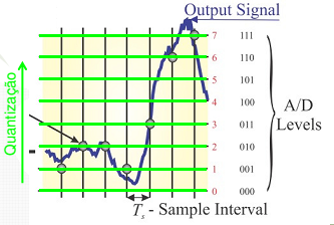
\includegraphics[height=5cm, keepaspectratio]{../figs/cap03/Imagem13}	
			\end{figure}
		\end{frame}
		
		\begin{frame}{Terminologia}
			\begin{itemize}
				\item Face sensora
				\begin{itemize}
					\item Lado do sensor que detecta o objeto
				\end{itemize}
				\vspace{.75em}
				\item Distância
				\begin{itemize}
					\item Espaço entre a face sensora e o objeto a ser detectado
				\end{itemize}
				\vspace{.75em}
				\item Histerese
			\end{itemize}
			\begin{figure}
				\centering
				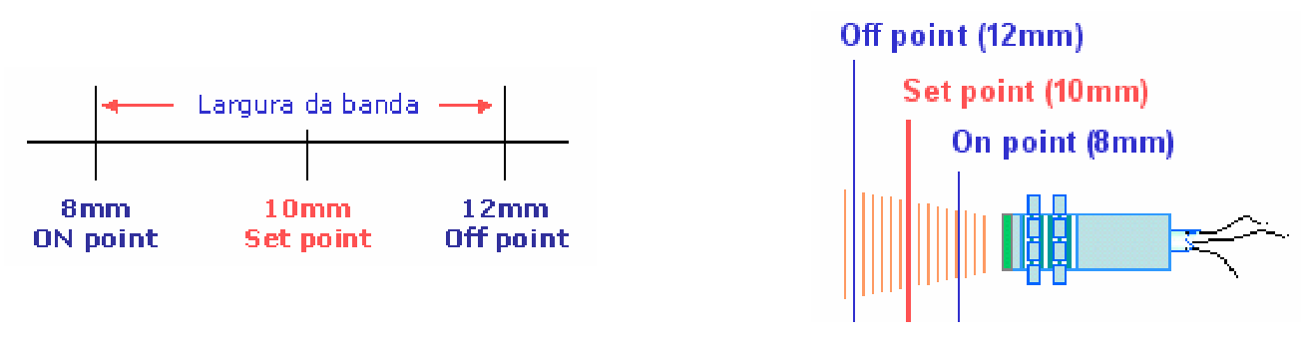
\includegraphics[scale=.4]{../figs/cap03/Imagem14}	
			\end{figure}
		\end{frame}
		
		\begin{frame}{Tipos de sensores}
			\begin{itemize}
				\item Mecânicos
				\vspace{.75em}
				\item Magnéticos – detectam apenas magnetos
				\vspace{.75em}
				\item Indutivos – apenas materiais ferromagnéticos
				\vspace{.75em}
				\item Capacitivos
				\vspace{.75em}
				\item Ópticos
				\vspace{.75em}
				\item Ultrassônicos
			\end{itemize}
		\end{frame}
		
		\begin{frame}{Sensores Mecânicos}
			\begin{itemize}
				\item Chaves de fim de curso
				\item Botoeiras
			\end{itemize}
			\begin{figure}
				\centering
				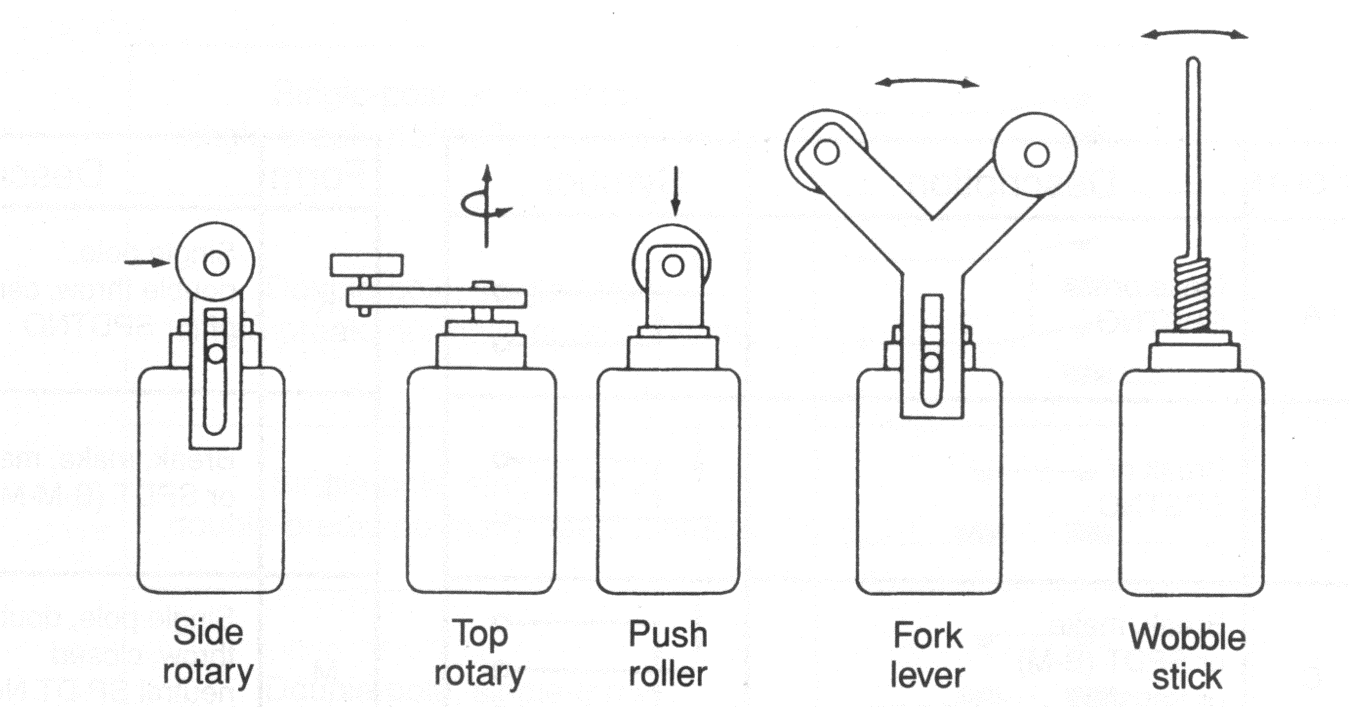
\includegraphics[scale=.4]{../figs/cap03/Imagem15}	
			\end{figure}
		\end{frame}	
		
		\begin{frame}{Sensores Mecânicos}
			\begin{itemize}
				\item Usados para medir quantidades como:
				\begin{itemize}
					\item Posição
					\item Velocidade
					\item Forma
					\item Força e torque
					\item Pressão
					\item Vibração, estresse
					\item Massa			
				\end{itemize}
			\end{itemize}
		\end{frame}
		
		\begin{frame}{Sensores indutivos}
			\begin{itemize}
				\item Variação na indutância gerada por uma bobina
			\end{itemize}
			\begin{figure}
				\centering
				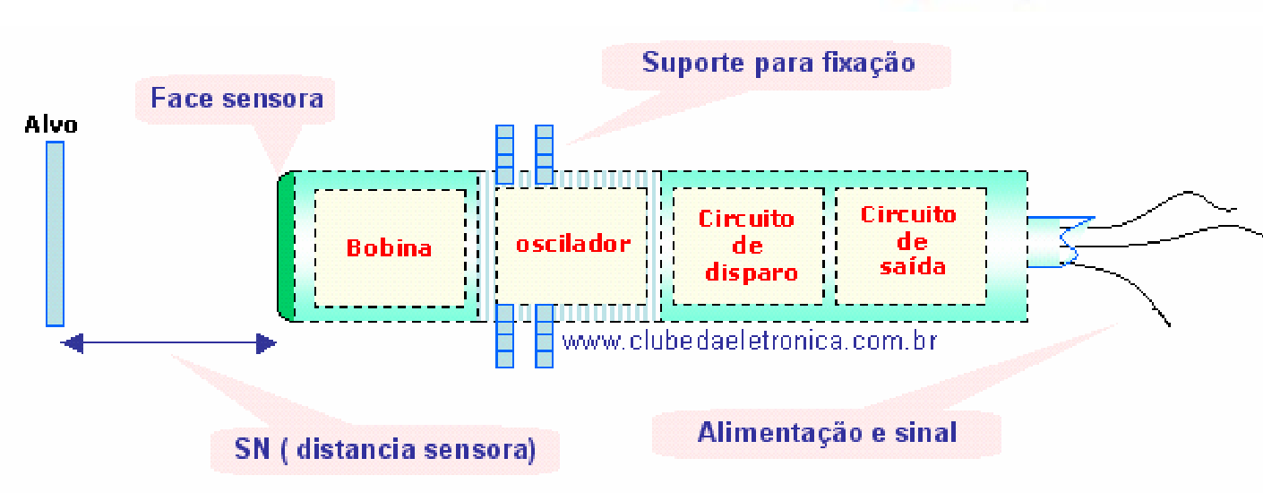
\includegraphics[scale=.4]{../figs/cap03/Imagem16}	
			\end{figure}		
		\end{frame}
		
		\begin{frame}{Princípio de Funcionamento}
			\begin{figure}
				\centering
				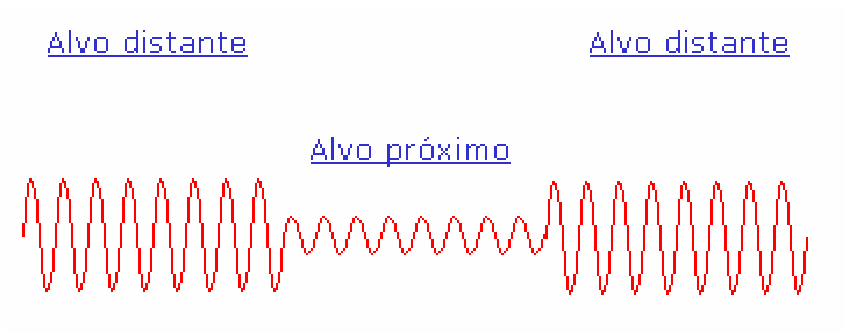
\includegraphics[scale=.4]{../figs/cap03/Imagem17}	
			\end{figure}			
		\end{frame}
		
%		\begin{frame}{Fator de correção}
%			\begin{figure}
%				\centering
%				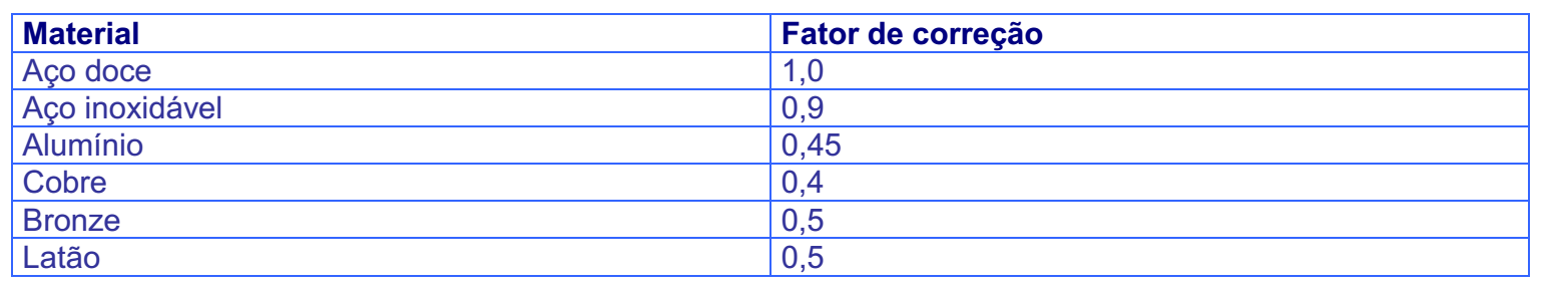
\includegraphics[scale=.4]{../figs/cap03/Imagem18}	
%			\end{figure}			
%		\end{frame}	
%		
%		\begin{frame}{Blindagem}
%			\begin{itemize}
%				\item Direcionamento do campo
%				\item Aumento da distância sensora e da precisão
%			\end{itemize}
%			\begin{figure}
%				\centering
%				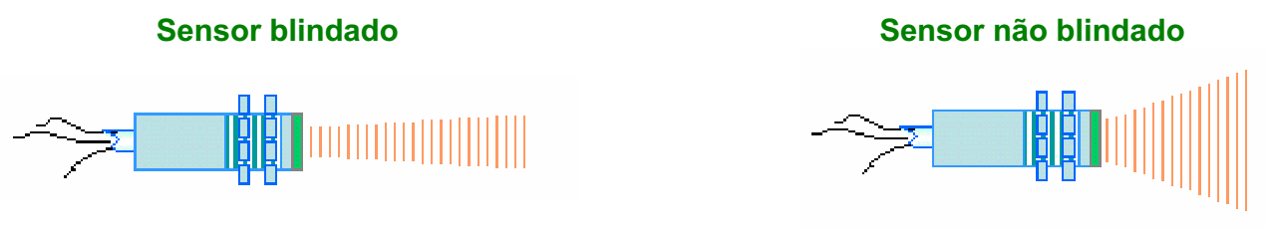
\includegraphics[scale=.4]{../figs/cap03/Imagem19}	
%			\end{figure}		
%		\end{frame}	
		
%		\begin{frame}{Embutimento}
%				\begin{table}
%					\centering
%					\begin{tabular}{m{0.5\textwidth} m{0.5\textwidth}}
%						\begin{itemize}
%							\item Embutido
%							\begin{itemize}
%								\begin{scriptsize}
%									\item Campo eletromagnético apenas na face sensora
%								\end{scriptsize}
%							\end{itemize}
%						\end{itemize}
%						&
%						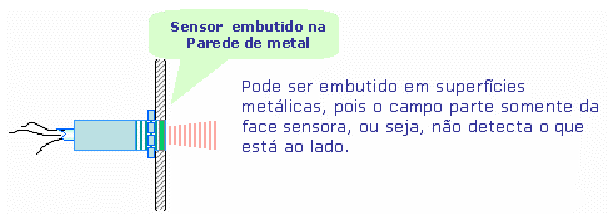
\includegraphics[scale=.33]{../figs/cap03/Imagem20} \\
%						\begin{itemize}
%							\item Não embutido
%							\begin{itemize}
%								\begin{scriptsize}
%									\item Campo eletromagnético na superfície da face sensora						
%								\end{scriptsize}
%							\end{itemize}
%						\end{itemize}
%						&
%						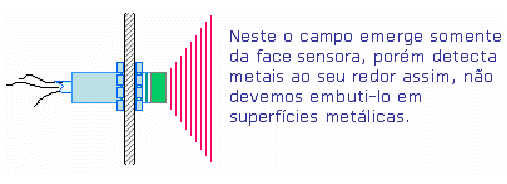
\includegraphics[scale=.33]{../figs/cap03/Imagem21} \\
%						\begin{itemize}
%							\item Semi-embutido
%							\begin{itemize}
%							\begin{scriptsize}
%								\item Campo magnético somente na face sensora, mas é afetado por metais ao redor						
%							\end{scriptsize}
%							\end{itemize}
%						\end{itemize}
%						& \\
%					\end{tabular}
%				\end{table}		
%		\end{frame}
		
		\begin{frame}{Sensores Capacitivos}
			\begin{itemize}
				\item Detectam objetos metálicos e não metálicos
				\vspace{0.8cm}
				\item Capacidade de detectar dentro de recipientes
				\vspace{0.8cm}
				\item Verificação de níveis de fluidos e sólidos em tanques
	
			\end{itemize}
	
			\begin{figure}
				\centering	
				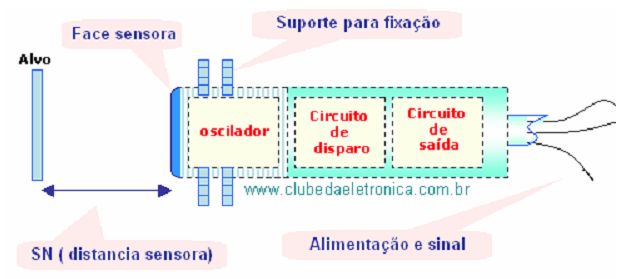
\includegraphics[scale=.5]{../figs/cap03/Imagem22}
			\end{figure}							
	
		\end{frame}
		
		\begin{frame}{Princípio de Funcionamento}
			\begin{figure}
				\centering	
				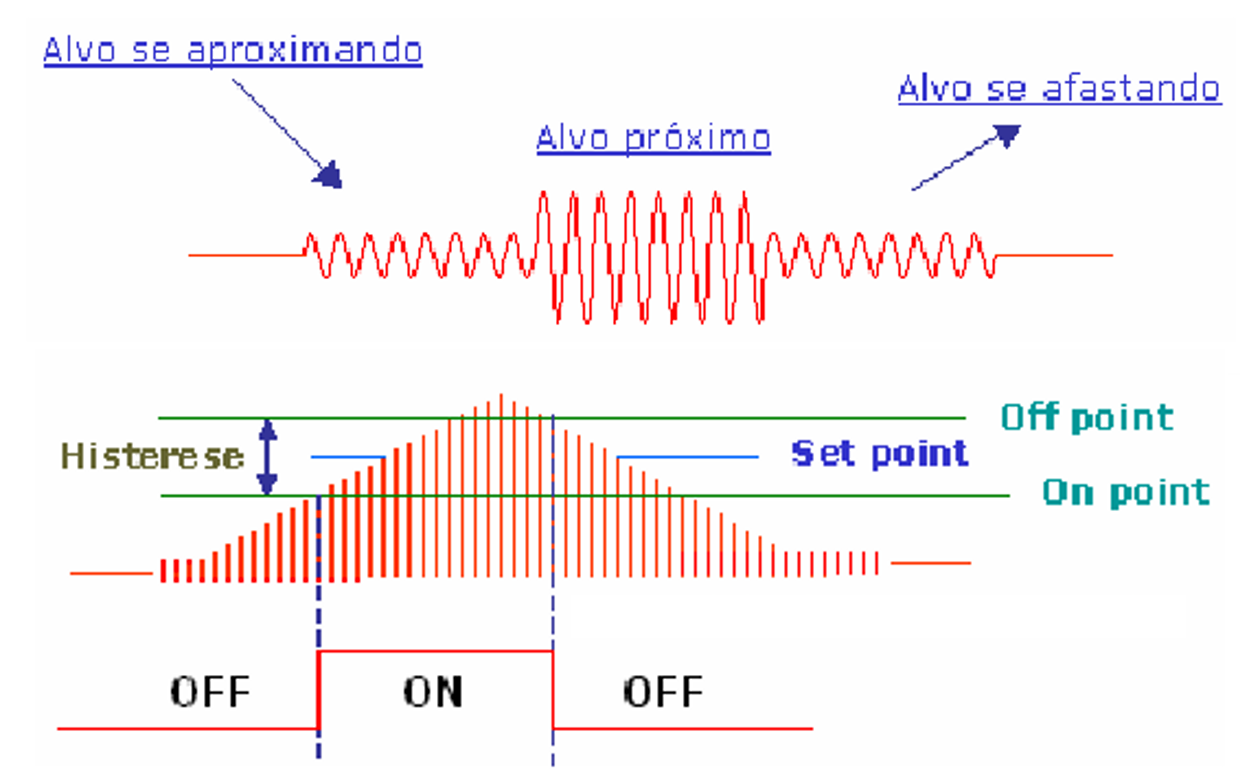
\includegraphics[scale=.35]{../figs/cap03/Imagem23}
			\end{figure}
		\end{frame}
	
		\begin{frame}{Constante dielétrica}
			\begin{figure}
				\centering	
				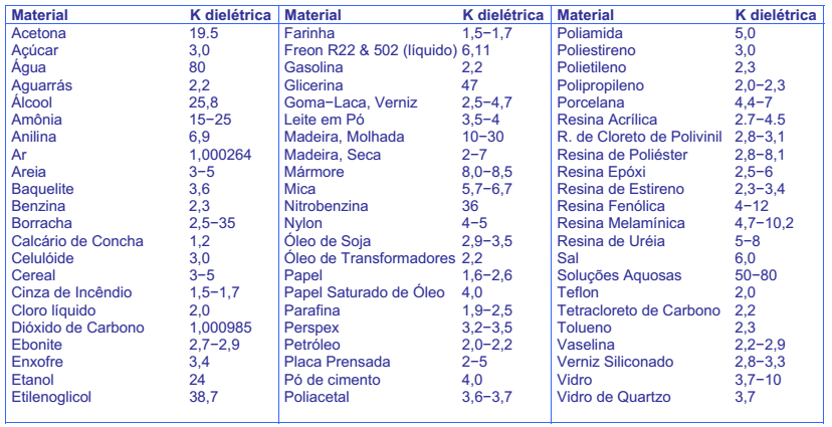
\includegraphics[scale=.45]{../figs/cap03/Imagem24}
			\end{figure}	
		\end{frame}		
	
		\begin{frame}{Sensores óticos}
			\begin{itemize}
				\item Emissão e recepção de feixes de luz 
				\vspace{0.8cm}
				\item Maior distância sensora
			\end{itemize}
			\begin{figure}
				\centering	
				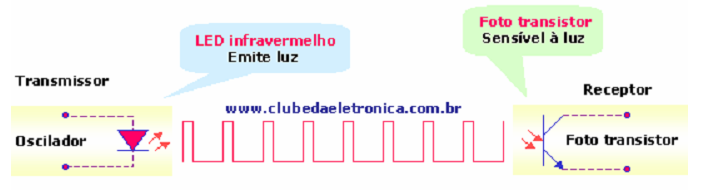
\includegraphics[scale=.5]{../figs/cap03/Imagem25}
			\end{figure}	
		\end{frame}
		
		\begin{frame}{Sensores óticos}
			\begin{itemize}
				\item Background
				\vspace{0.5cm}
				\item Zona Morta
				\vspace{0.5cm}
				\item Interferências do meio
				\vspace{0.5cm}
				\item Fator de correção
			\end{itemize}
			\begin{figure}
				\centering	
				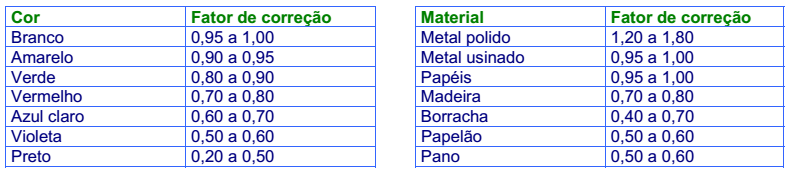
\includegraphics[scale=.5]{../figs/cap03/Imagem26}
			\end{figure}	
		\end{frame}
		
		\begin{frame}{Sensores ultrassônicos}
			\begin{itemize}
				\item Emissão e recepção de ondas sonoras
			\end{itemize}
			\begin{figure}
				\centering	
				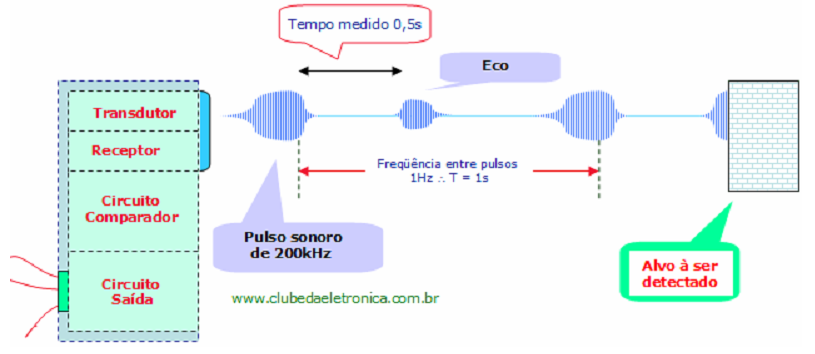
\includegraphics[scale=.5]{../figs/cap03/Imagem27}
			\end{figure}	
		\end{frame}
		
		\begin{frame}{Princípio de funcionamento}
			\begin{figure}
				\centering	
				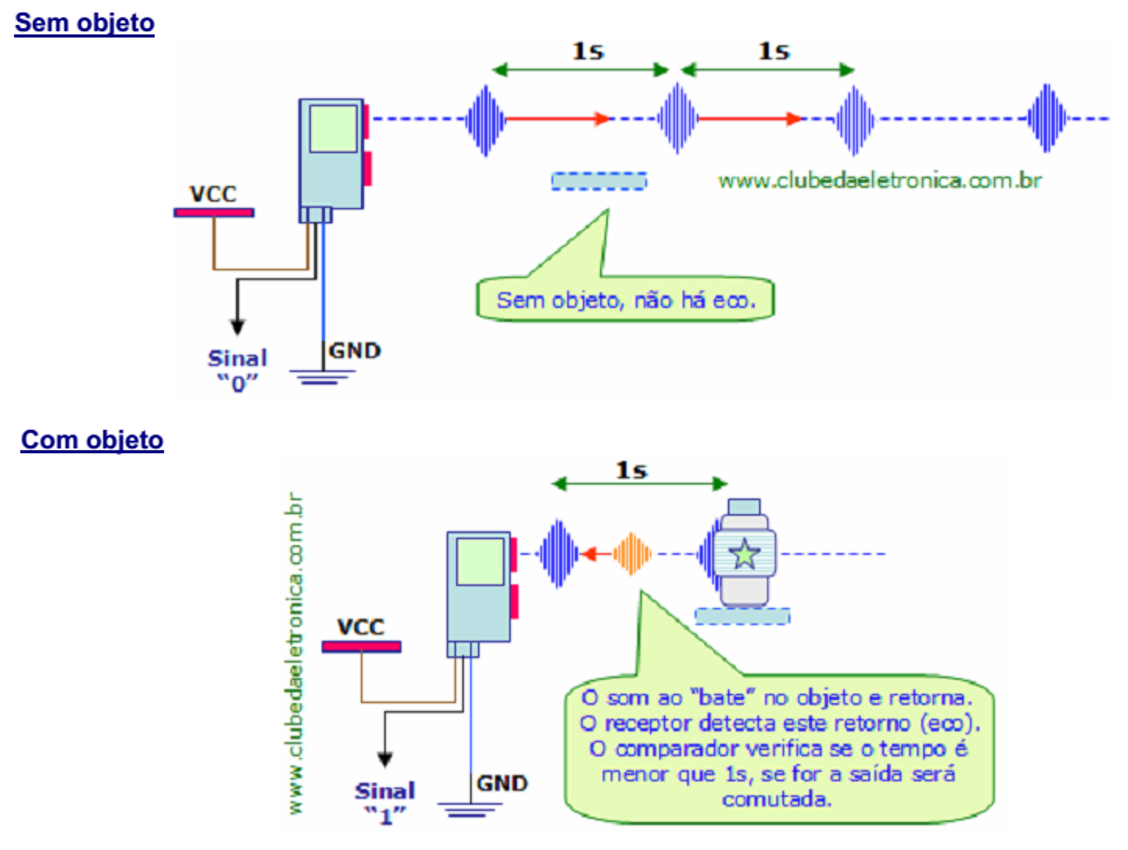
\includegraphics[scale=.25]{../figs/cap03/Imagem28}
			\end{figure}	
		\end{frame}
		
		\begin{frame}{Sensores segundo a função}
			\begin{itemize}
					\item Manipulação
					\begin{itemize}
						\item Que interagem com o meio ambiente do robô. 
						\item Ex: sensores de Força.
					\end{itemize}
					\vspace{0.8cm}
					\item Aquisição
					\begin{itemize}
						\item Que permitem ao robô perceber seu próprio estado.
						\item Ex: encoders.				
					\end{itemize}
			\end{itemize}
		\end{frame}	
		
		\begin{frame}{Sensores segundo a localização}
				\begin{itemize}
					\item Internos
					\begin{itemize}
						\item Encoders.				
					\end{itemize}
				\vspace{0.8cm}
					\item Externos
					\begin{itemize}
						\item Swiches, táteis, proximidade e fotoelétricos.
					\end{itemize}
				\vspace{0.8cm}
					\item \textit{Interlocked}
					\begin{itemize}
						\item Usados para proteger o robô.
						\item Travam o robô até que certa condição se torne válida (pressão de fluido, temperatura alta, etc)
					\end{itemize}
				\end{itemize}
		\end{frame}		
	
		\begin{frame}{Sensores segundo a ativação}
			\begin{itemize}
					\item Contato
					\begin{itemize}
						\item Existe um contato físico para a ativação
						\item Ex.: switches				
					\end{itemize}
				\vspace{0.8cm}
					\item Sem contato
					\begin{itemize}
						\item Não existe um contato físico para a ativação
						\item Ex.: visão, ultrassom, radiação
					\end{itemize}
			\end{itemize}
		\end{frame}			
		
		\begin{frame}
			\begin{figure}
				\centering	
				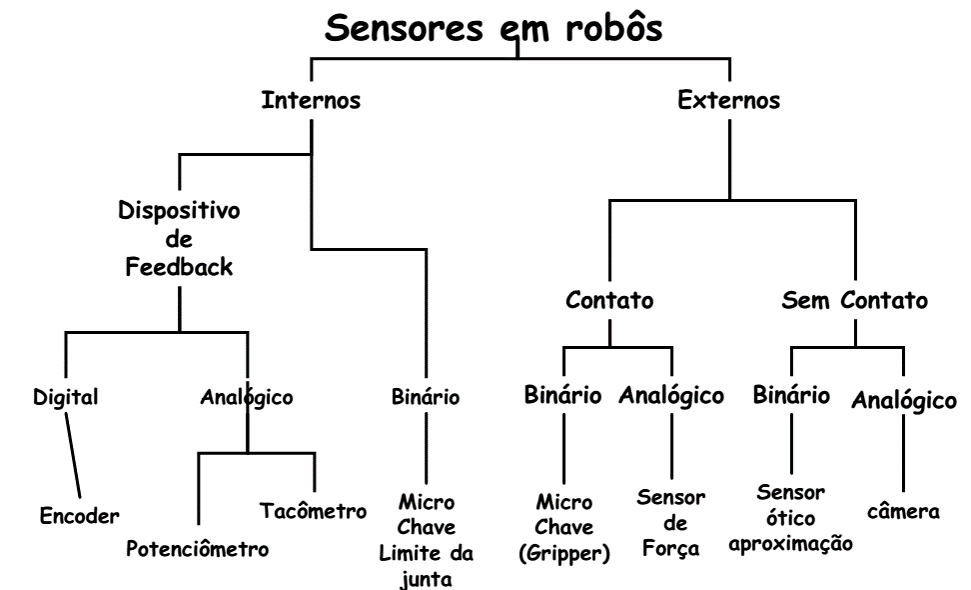
\includegraphics[scale=.4]{../figs/cap03/Imagem29}
			\end{figure}	
		\end{frame}			
		
		\begin{frame}{Classificação - Aplicação}
			\begin{itemize}
				\item Proximidade
				\vspace{0.8cm}	
				\item Posição / Velocidade
				\vspace{0.8cm}	
				\item Força / pressão
				\vspace{0.8cm}	
				\item Vibração / Aceleração
				\vspace{0.8cm}	
				\item Tato
	
			\end{itemize}			
		
		\end{frame}
		
		\begin{frame}{Sensores de Proximidade}
			\begin{itemize}
				\item On / Off – presença ou ausência de objeto
	
				\item Tipos
				\begin{itemize}
					\item Chave mecânica
					\item Ótico
					\item Ultrassônico
					\item Indutivo
					\item Capacitivo			
				\end{itemize}
			\end{itemize}				
		\end{frame}
		
		\begin{frame}{Sensores de Proximidade}
			\begin{itemize}
				\item É necessário, em geral, pelo menos duas funções de segurança:
				\begin{enumerate}
					\item Desligar ou poder desabilitar quando uma pessoa entra na área de perigo.	
					\item Evitar ligar ou habilitação de força quando uma pessoa está na zona de perigo.
					
				\end{enumerate}
			\end{itemize}
		\end{frame}
		
		\begin{frame}{Cortinas de luz}
			\begin{columns}
				\column{0.7\textwidth}
				\begin{itemize}
					\item As cortinas de luz de segurança são sensores de presença fotoelétrico projetados especificamente para proteger o pessoal de lesões relacionadas com o movimento da máquina perigosa. 
				\vspace{0.8cm}
					\item Também conhecido como: 
					\begin{itemize}
						\item AOPDs (dispositivos de proteção individual optoeletrônicos ativos)  
						\item ESPE (equipamentos de proteção individual eletrosensiveis)
					\end{itemize}
				\end{itemize}
				\column{0.3\textwidth}
				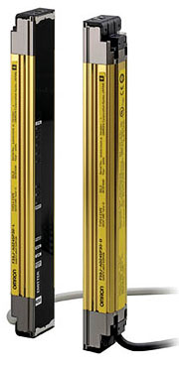
\includegraphics[scale=.4]{../figs/cap03/Imagem30}
	
			\end{columns}
		\end{frame}
	
	%	Vídeo
	%	\begin{frame}
	%		\begin{figure}[ht]
	%			\includemovie[poster]{6cm}{4cm}{midia1.mp4}
	%		\end{figure}
	%	\end{frame}
	
		\begin{frame}{Scanners a laser}
			\begin{itemize}
				\item Os leitores de segurança a laser usam um espelho rotativo que criam um plano de detecção. 
				\vspace{0.8cm}
				\item A localização do objeto é determinado pelo ângulo de rotação do espelho e pelo “tempo de vôo” de um feixe de laser.
				\begin{itemize}
					\item Ao tomar a medida da distância e da localização do objeto, o scanner a laser determina a posição exata do objeto. 
				\end{itemize}
			\end{itemize}
		\end{frame}
		
		\begin{frame}{Scanners a laser}
			\begin{itemize}
				\item Os scanners a laser criam duas zonas
				\begin{enumerate}
					\item uma zona de alerta: fornece um sinal de que não desliga o perigo e informa às pessoas que elas estão se aproximando da zona de segurança 
					\item uma zona de segurança: quando um objeto entra, faz o scanner a laser emitir uma ordem de parada; as saídas dos controladores se desligam.
				\end{enumerate}
			\end{itemize}
		\end{frame}
		
		\begin{frame}{Scanners a laser}
			\centering
			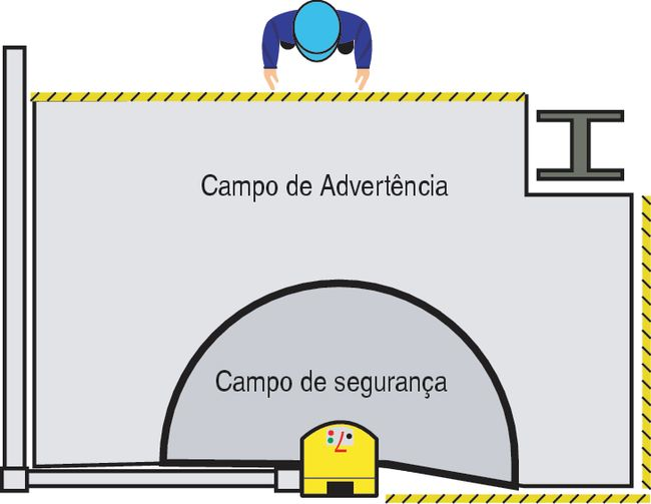
\includegraphics[scale=.5]{../figs/cap03/Imagem31}
		\end{frame}
		
		\begin{frame}{Tapetes de segurança sensíveis a pressão}
			\begin{itemize}
				\item Usados para a vigilância de uma área em torno de uma máquina
				\vspace{0.8cm}
				\item Uma matriz de tapetes interligados é definido em torno da área de risco e a pressão aplicada ao tapete (por exemplo, passos de um operador) fará com que a unidade controladora do tapete desligue a alimentação do perigo. 
			\end{itemize}
		\end{frame}
		
		\begin{frame}{Tapetes de Segurança}
			\centering
			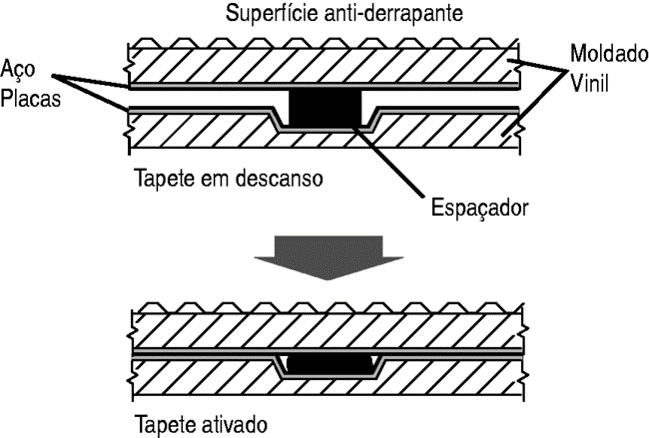
\includegraphics[scale=.5]{../figs/cap03/Imagem32}		
		\end{frame}
		
		\begin{frame}{Tapetes de Segurança}
			\centering
			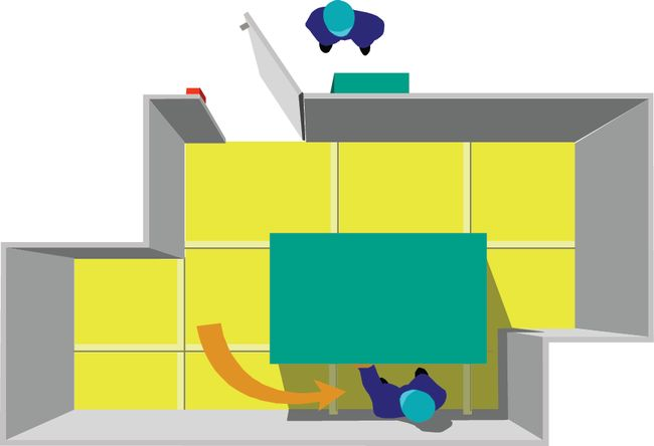
\includegraphics[scale=.5]{../figs/cap03/Imagem33}		
		\end{frame}	
		
		\begin{frame}{Sensores de Velocidade / Aceleração}
			\begin{itemize}
				\item Sensores de velocidade
				\begin{itemize}
					\item Potenciômetro
					\item LVDT
					\item Encoder			
				\end{itemize}
				\item Sensores de aceleração
				\begin{itemize}
					\item Tacômetro			
				\end{itemize}
			\end{itemize}
		\end{frame}
		
		\begin{frame}{Potenciômetro}
			\begin{itemize}
				\item Resistor variável
				\item Vantagens
				\begin{itemize}
					\item Simples
					\item Barato			
				\end{itemize}
				\item Desvantagens
				\begin{itemize}
					\item Pouco exato
					\item Baixa resolução			
				\end{itemize}
			\end{itemize}
		\end{frame}
		
		\begin{frame}{LVDT (\textit{Linear Variable Differential Transformer})}
			\begin{itemize}
				\item Um LVDT consiste de um núcleo magnético que move dentro de um cilindro
				\item A luva do cilindro contém uma bobina primária com uma tensão oscilante aplicada
				\item A luva também contém dois secundários que detectam esta tensão com a magnitude igual ao deslocamento
				\item LVDTs são muito precisos (centésimo de milímetro)
			\end{itemize}
			\begin{figure}
				\centering
				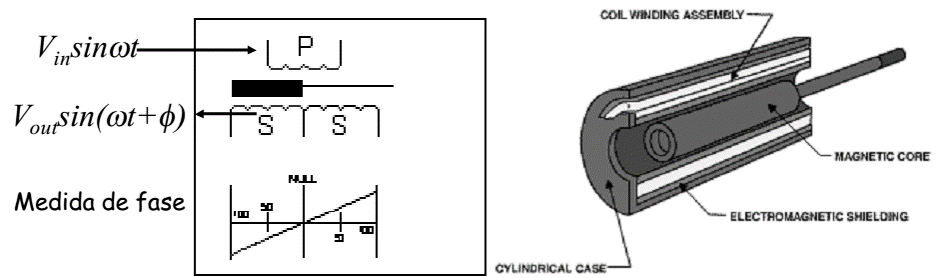
\includegraphics[scale=.35]{../figs/cap03/Imagem34}			
			\end{figure}
		\end{frame}
		
		\begin{frame}{\textit{Encoders}}
			\begin{itemize}
				\item \textit{Encoders} são sensores digitais usados para dar \textit{feedback} de posição para atuadores
				\item Consiste de um disco de vidro ou plástico que gira entre uma fonte de luz (LED) e um par de fotodetectores
				\item O disco é marcado com setores ou riscos que bloqueiam a passagem da luz, produzindo pulsos conforme gira
			\end{itemize}
			\begin{figure}
				\centering
				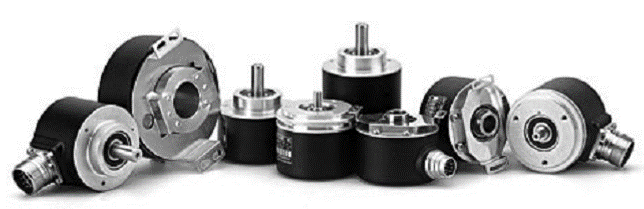
\includegraphics[scale=.35]{../figs/cap03/Imagem35}			
			\end{figure}	
		\end{frame}
		
		\begin{frame}{Codificação}
			\begin{figure}
				\centering
				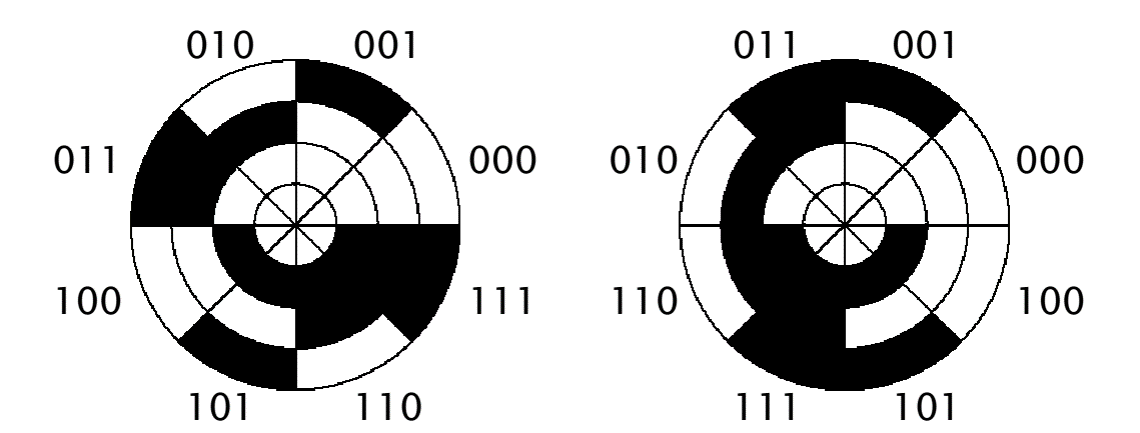
\includegraphics[scale=.35]{../figs/cap03/Imagem40}			
			\end{figure}			
		\end{frame}
		
		\begin{frame}{\textit{Resolvers}}
			\begin{itemize}
				\item Sensor de posição absoluta
				\begin{itemize}
					\item Um estator composto por dois enrolamentos, A e B.
					\item O enrolamento A está posicionado a 90 graus do enrolamento B.
					\item O rotor é composto por um terceiro enrolamento, C, que é energizado com uma onda senoidal.
					\item O sinal em C induz sinais em A e B, que variam com a posição angular de C.
					\item A voltagem induzida em A está em quadratura com a de B.
					\item Cada posição do rotor produz valores diferentes em A e B.
				\end{itemize}
			\end{itemize}
		\end{frame}
	
		\begin{frame}{\textit{Resolvers}}
			\begin{figure}
				\centering
				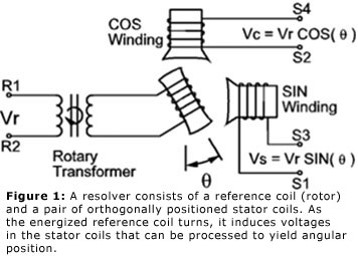
\includegraphics[scale=.35]{../figs/cap03/Imagem41.jpg}			
			\end{figure}			
		\end{frame}
		
		\begin{frame}{\textit{Resolvers}}
			\begin{figure}
				\centering
				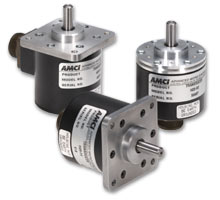
\includegraphics[scale=.5]{../figs/cap03/Imagem42}	
				\hspace{0.5cm}
				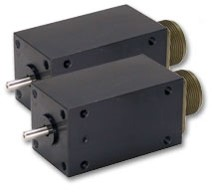
\includegraphics[scale=.5]{../figs/cap03/Imagem43}		
			\end{figure}			
		\end{frame}
		
		\begin{frame}{Tacômetro}
			\begin{itemize}
				\item Medida de velocidade de rotação utilizando um gerador DC
				\item Essencialmente é um motor girando ao contrário
				\item Normalmente utiliza-se conectados diretamente ao motor para se ter \textit{feedback}
			\end{itemize}
			\begin{figure}
				\centering
				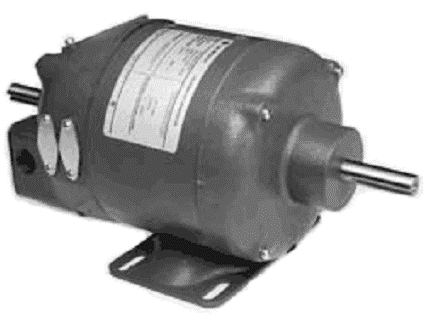
\includegraphics[scale=.4]{../figs/cap03/Imagem44}			
			\end{figure}	
		\end{frame}
		\begin{frame}{}
		\end{frame}
\end{document}
